\clearpage
\chapter{Mastery Workbook 9}

% Chapter page
\section{Counting And Binomials Workbook}

\horizontalline{0}{0}

\begin{center}
    \Large{\textbf{I have neither given nor received unauthorized assistance.}}
    \horizontalline{0}{0}
    \large{\textbf{Taylor James Larrechea}}
    \horizontalline{0}{0}
\end{center}

% Problem 1
\begin{problem}{Problem 1}
    \begin{statement}{Problem Statement}
        Problem 1 from the mastery workbook quiz can be found on the following page.
    \end{statement}
    \begin{Highlight}[Solution]
        \begin{center}
            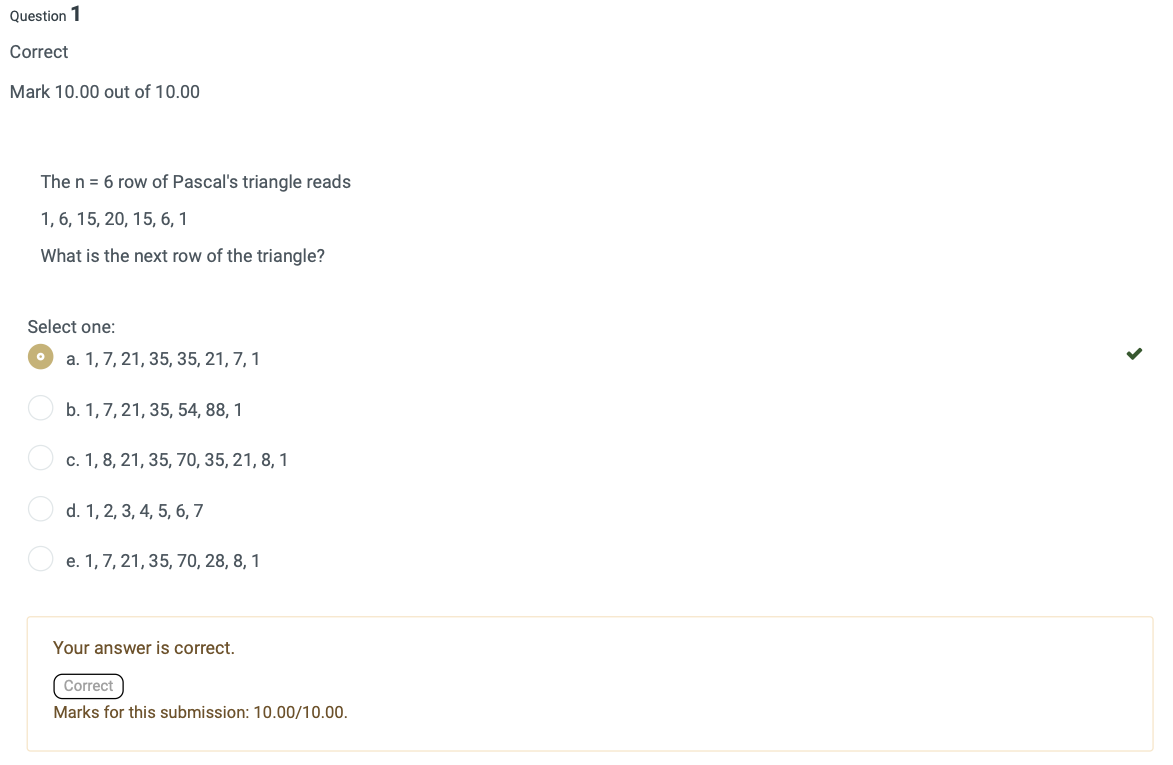
\includegraphics[width = 1.0\textwidth]{Images/Problem 1.png}
        \end{center}
    \end{Highlight}
\end{problem}

% Problem 1 Summary
\begin{summary}{Problem 1 Summary}
    \begin{statement}{Procedure}
        \begin{itemize}
            \item Read off the $n = 7$ line of Pascals triangle and select the corresponding answer.
        \end{itemize}
    \end{statement}
    \begin{statement}{Key Concepts}
        \begin{itemize}
            \item This problem showcases Pascals triangle and what the rows of his triangle are.
        \end{itemize}
    \end{statement}
    \begin{statement}{Variations}
        \begin{itemize}
            \item We could be asked to select a different row from Pascals triangle.
            \begin{itemize}
                \item In that case we would just look at Pascals triangle and select the correct row.
            \end{itemize}
        \end{itemize}
    \end{statement}
\end{summary}

% Problem 2
\begin{problem}{Problem 2}
    \begin{statement}{Problem Statement}
        Problem 2 from the mastery workbook quiz can be found on the following page.
    \end{statement}
    \begin{Highlight}[Solution]
        \begin{center}
            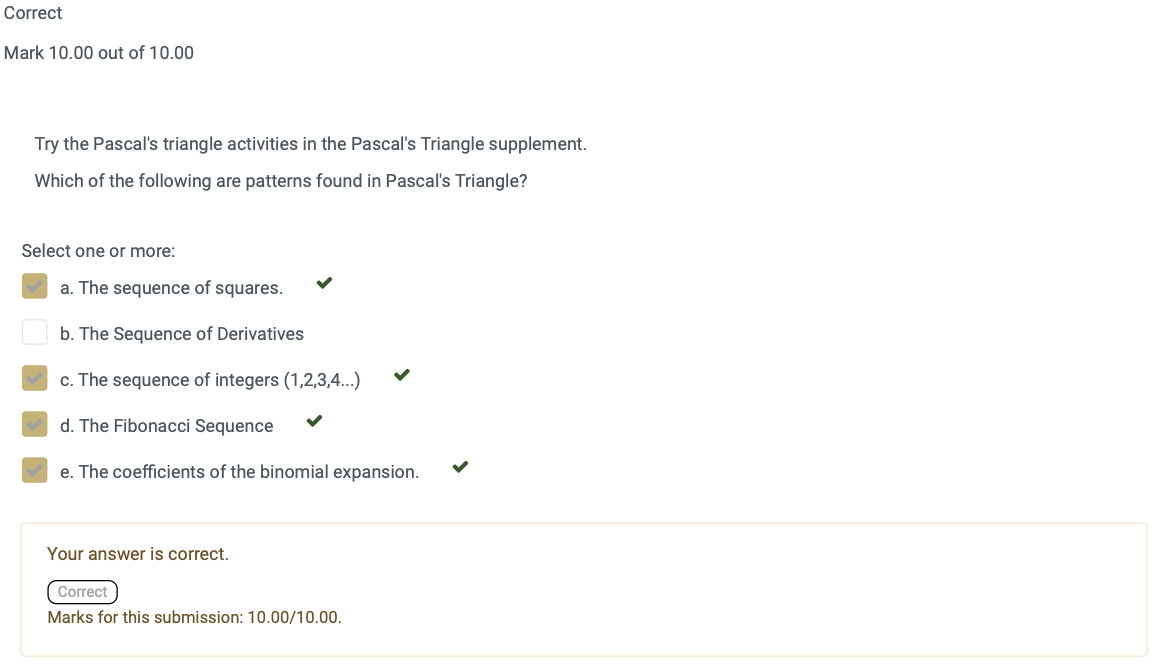
\includegraphics[width = 1.0\textwidth]{Images/Problem 2.png}
        \end{center}
    \end{Highlight}
\end{problem}

% Problem 2 Summary
\begin{summary}{Problem 2 Summary}
    \begin{statement}{Procedure}
        \begin{itemize}
            \item Observe Pascals triangle and look at the patterns inside of Pascals triangle.
            \item Select the correct options from the given choices.
        \end{itemize}
    \end{statement}
    \begin{statement}{Key Concepts}
        \begin{itemize}
            \item Pascals triangle shows a sequence of squares.
            \item Pascals triangle shows a sequence of integers.
            \item Pascals triangle shows the Fibonacci sequence.
            \item Pascals triangle shows the coefficients of the binomial expansion.
        \end{itemize}
    \end{statement}
    \begin{statement}{Variations}
        \begin{itemize}
            \item We could be asked to examine different patterns inside of Pascals triangle.
            \begin{itemize}
                \item We would then have to sift through the choices to see which ones are the correct answers.
            \end{itemize}
        \end{itemize}
    \end{statement}
\end{summary}

% Problem 3
\begin{problem}{Problem 3}
    \begin{statement}{Problem Statement}
        Problem 3 from the mastery workbook quiz can be found on the following page.
    \end{statement}
    \begin{Highlight}[Solution]
        \begin{center}
            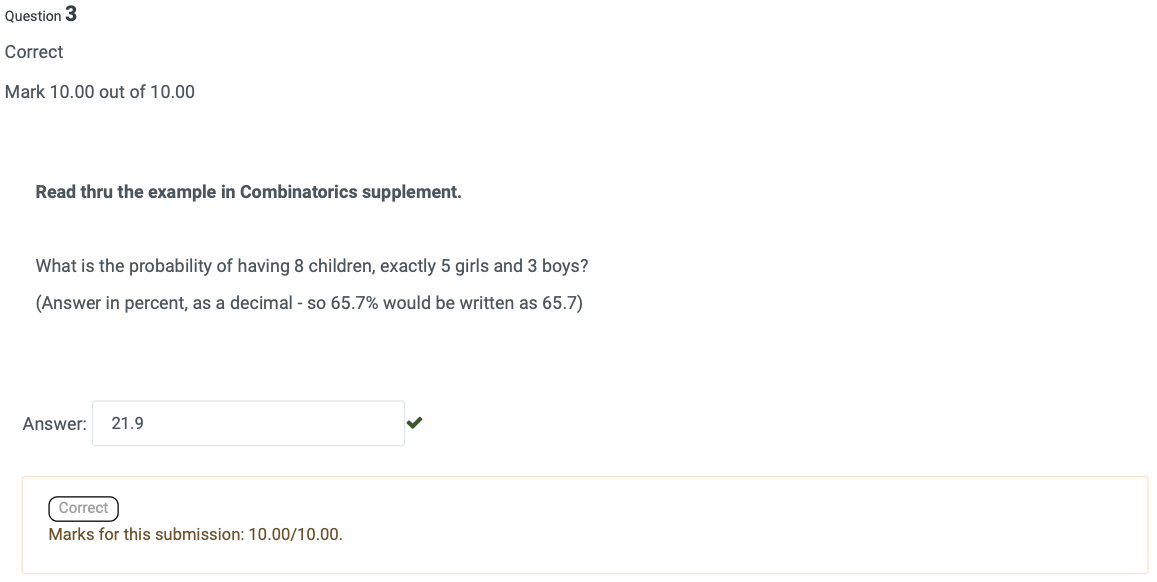
\includegraphics[width = 1.0\textwidth]{Images/Problem 3.png}
        \end{center}
    \end{Highlight}
\end{problem}

% Problem 3 Summary
\begin{summary}{Problem 3 Summary}
    \begin{statement}{Procedure}
        \begin{itemize}
            \item Calculate the overall probability from having 8 children, namely
            \begin{equation*}
                \Biggl(\frac{1}{2}\Biggr)^{8}.
            \end{equation*}
            \item Read off the column value from Pascals triangle for there to be 5 out of 8 binary possibilities.
            \item Multiply this value (56) by $(\frac{1}{2})^{8}$ to get the overall probability.
        \end{itemize}
    \end{statement}
    \begin{statement}{Key Concepts}
        \begin{itemize}
            \item This problem showcases how we can use Pascals triangle to calculate binary choice probabilities.
        \end{itemize}
    \end{statement}
    \begin{statement}{Variations}
        \begin{itemize}
            \item We could be asked to calculate the probability of a different number of children (or binary choices) being born with different values for girls and boys.
            \begin{itemize}
                \item We would then use the same framework of the problem, read off the value from Pascals triangle, and perform similar calculations.
            \end{itemize}
        \end{itemize}
    \end{statement}
\end{summary}

% Problem 4
\begin{problem}{Problem 4}
    \begin{statement}{Problem Statement}
        Problem 4 from the mastery workbook quiz can be found on the following page.
    \end{statement}
    \begin{Highlight}[Solution]
        \begin{center}
            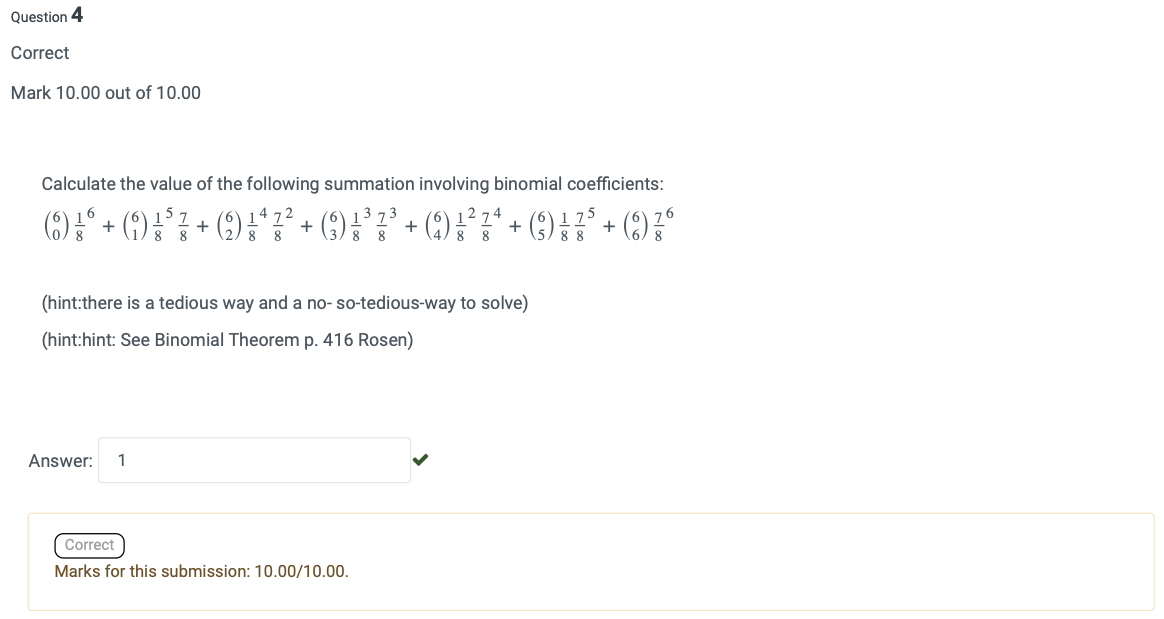
\includegraphics[width = 1.0\textwidth]{Images/Problem 4.png}
        \end{center}
    \end{Highlight}
\end{problem}

% Problem 4 Summary
\begin{summary}{Problem 4 Summary}
    \begin{statement}{Procedure}
        \begin{itemize}
            \item Use the Binomial Theorem, namely
            \begin{equation*}
                (x + y)^{n} = \sum_{k = 0}^{n} {n \choose k}x^{n - k}y^{k}
            \end{equation*}
            where the choose formula is 
            \begin{equation*}
                {n \choose k} = \frac{n!}{k!(n - k)!}
            \end{equation*}
            where $x = \frac{1}{8}$, $y = \frac{7}{8}$, and $n = 6$.
            \item Round the final answer from the Binomial Theorem result.
        \end{itemize}
    \end{statement}
    \begin{statement}{Key Concepts}
        \begin{itemize}
            \item The Binomial Theorem can be used to calculate a complex sum in this context.
            \item In this context, the value for $x$ and $y$ represent the the coefficients in front of two variables that are being summed and raised to a power.
        \end{itemize}
    \end{statement}
    \begin{statement}{Variations}
        \begin{itemize}
            \item We could be given a different expression to evaluate with the Binomial Theorem.
            \begin{itemize}
                \item We would then use the Binomial theorem to determine what this new sum evaluates to.
            \end{itemize}
        \end{itemize}
    \end{statement}
\end{summary}

% Problem 5
\begin{problem}{Problem 5}
    \begin{statement}{Problem Statement}
        Problem 5 from the mastery workbook quiz can be found on the following page.
    \end{statement}
    \begin{Highlight}[Solution]
        \begin{center}
            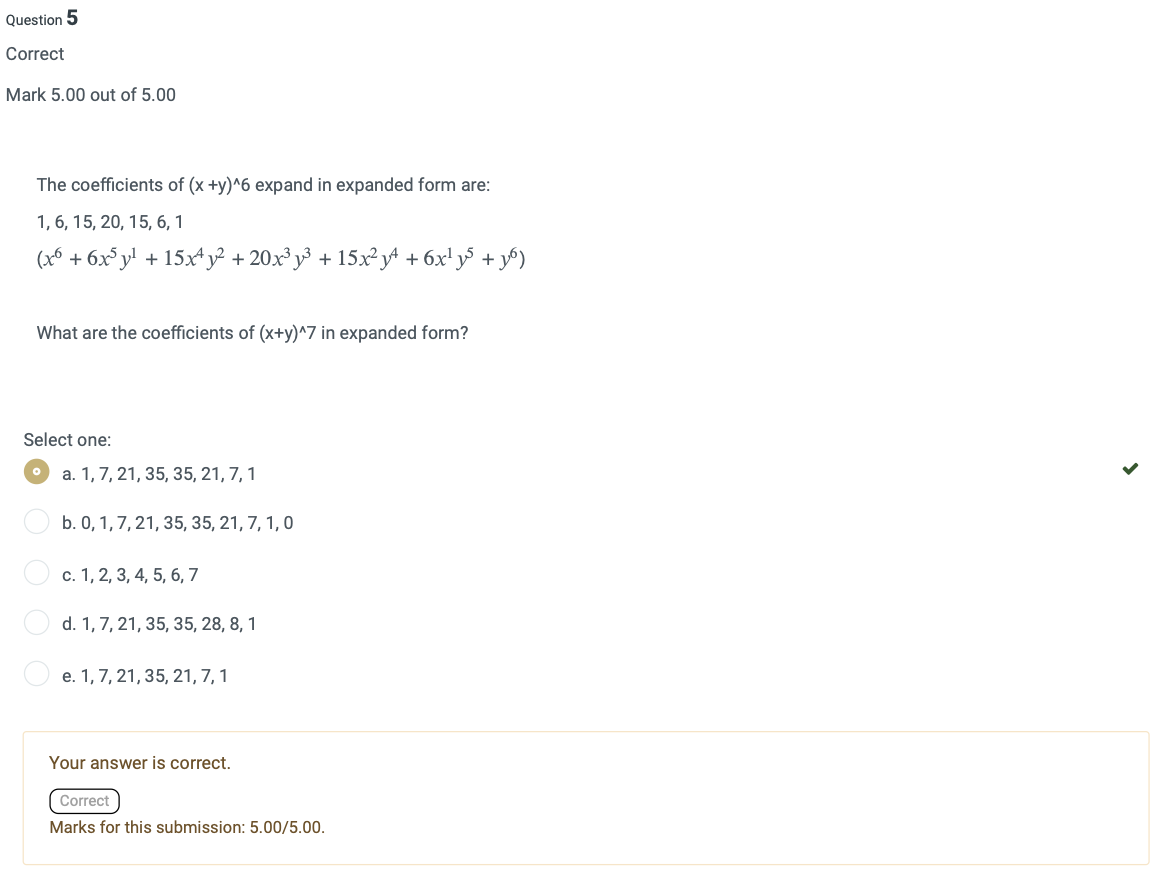
\includegraphics[width = 1.0\textwidth]{Images/Problem 5.png}
        \end{center}
    \end{Highlight}
\end{problem}

% Problem 5 Summary
\begin{summary}{Problem 5 Summary}
    \begin{statement}{Procedure}
        \begin{itemize}
            \item Determine the value of the exponent that is being used in the Binomial Theorem.
            \item Go to this line of Pascals triangle and choose the correct choice.
        \end{itemize}
    \end{statement}
    \begin{statement}{Key Concepts}
        \begin{itemize}
            \item This problem encapsulates determining what row of Pascals triangle is present in the expansion.
        \end{itemize}
    \end{statement}
    \begin{statement}{Variations}
        \begin{itemize}
            \item We could be given a different expansion to decide which row of Pascals triangle is being shown.
            \begin{itemize}
                \item We would then just read off of Pascals triangle what row is being represented.
            \end{itemize}
        \end{itemize}
    \end{statement}
\end{summary}

% Problem 6
\begin{problem}{Problem 6}
    \begin{statement}{Problem Statement}
        Problem 6 from the mastery workbook quiz can be found on the following page.
    \end{statement}
    \begin{Highlight}[Solution]
        \begin{center}
            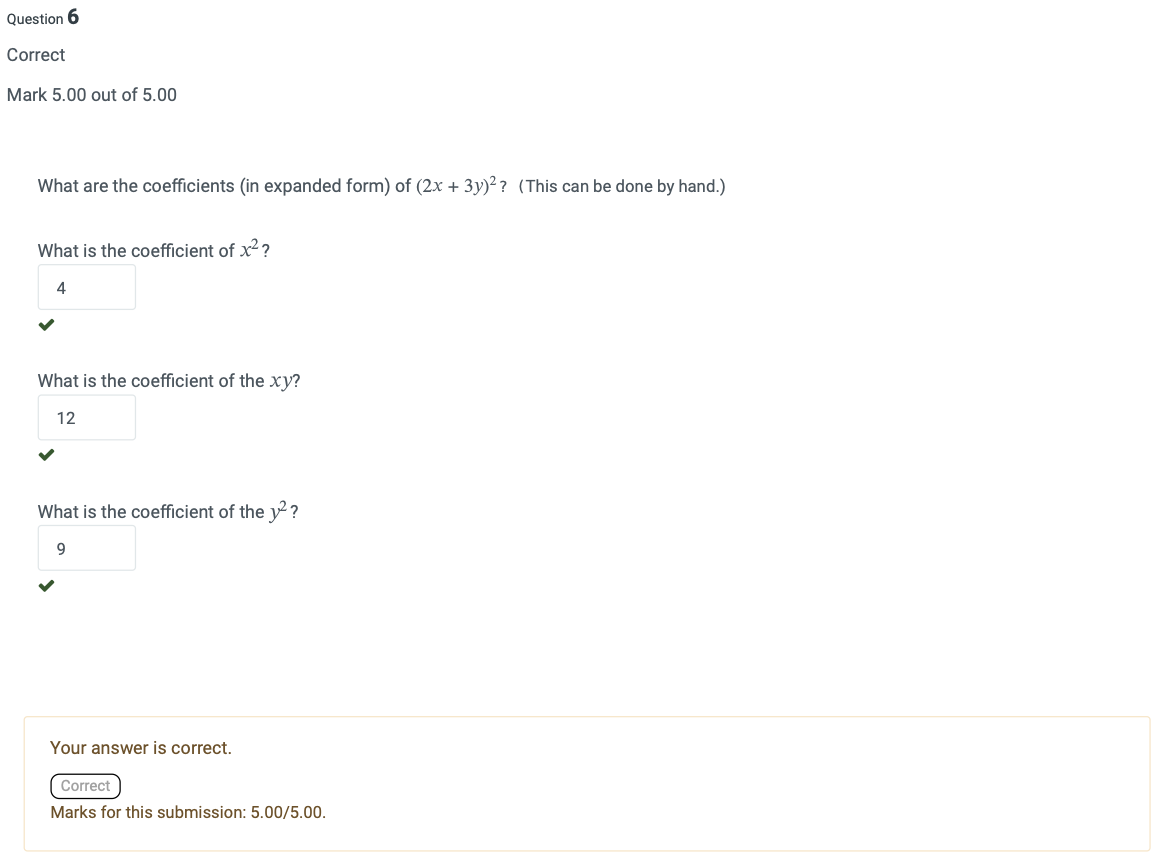
\includegraphics[width = 1.0\textwidth]{Images/Problem 6.png}
        \end{center}
    \end{Highlight}
\end{problem}

% Problem 6 Summary
\begin{summary}{Problem 6 Summary}
    \begin{statement}{Procedure}
        \begin{itemize}
            \item Expand the expression.
            \item Read off the coefficients from the expansion and submit the correct choices.
        \end{itemize}
    \end{statement}
    \begin{statement}{Key Concepts}
        \begin{itemize}
            \item This problem encapsulates how the Binomial Theorem can be used to find the coefficients in an expansion.
        \end{itemize}
    \end{statement}
    \begin{statement}{Variations}
        \begin{itemize}
            \item We could be given a different expression to calculate the coefficients for.
            \begin{itemize}
                \item We would then use the Binomial Theorem to calculate the coefficients for the expansion. Or just do it by hand if it is simple enough.
            \end{itemize}
        \end{itemize}
    \end{statement}
\end{summary}

% Problem 7
\begin{problem}{Problem 7}
    \begin{statement}{Problem Statement}
        Problem 7 from the mastery workbook quiz can be found on the following page.
    \end{statement}
    \begin{Highlight}[Solution]
        \begin{center}
            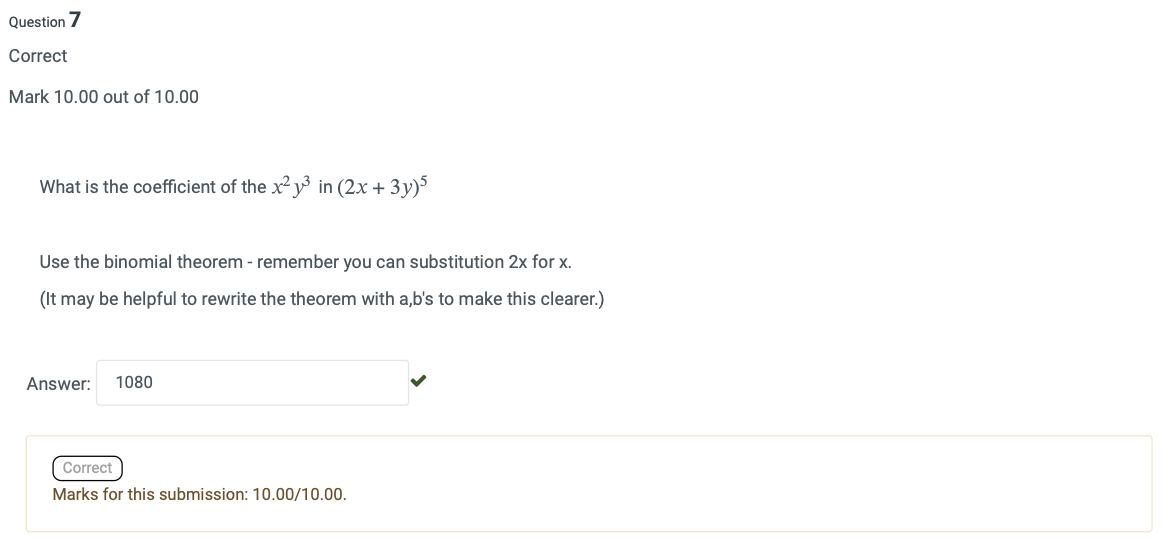
\includegraphics[width = 1.0\textwidth]{Images/Problem 7.png}
        \end{center}
    \end{Highlight}
\end{problem}

% Problem 7 Summary
\begin{summary}{Problem 7 Summary}
    \begin{statement}{Problem Statement}
        \begin{itemize}
            \item Use the Binomial Theorem where $x = 2$, $y = 3$, and $n = 5$.
            \item Read off the coefficient from the $x^{2}y^{3}$ term.
        \end{itemize}
    \end{statement}
    \begin{statement}{Key Concepts}
        \begin{itemize}
            \item This problem incorporates how to use the Binomial Theorem for an expansion.
        \end{itemize}
    \end{statement}
    \begin{statement}{Variations}
        \begin{itemize}
            \item We could be given a different expression to find the coefficients for.
            \begin{itemize}
                \item We would then use the Binomial Theorem for this new expression and read off the correct coefficients.
            \end{itemize}
        \end{itemize}
    \end{statement}
\end{summary}

% Problem 8
\begin{problem}{Problem 8}
    \begin{statement}{Problem Statement}
        Problem 8 from the mastery workbook quiz can be found on the following page.
    \end{statement}
    \begin{Highlight}[Solution]
        \begin{center}
            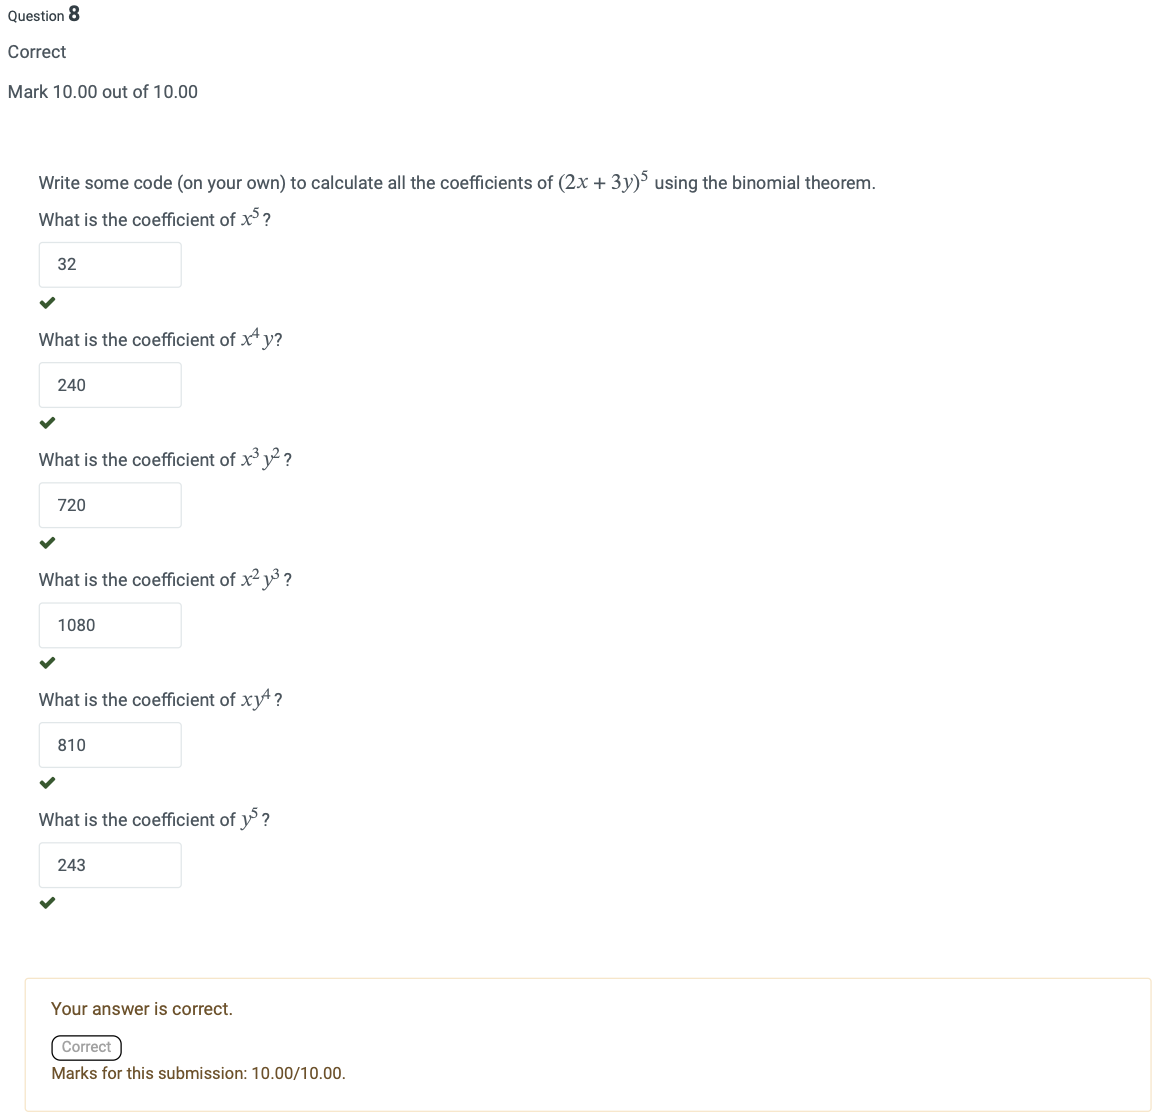
\includegraphics[width = 1.0\textwidth]{Images/Problem 8.png}
        \end{center}
    \end{Highlight}
\end{problem}

% Problem 8 Summary
\begin{summary}{Problem 8 Summary}
    \begin{statement}{Procedure}
        \begin{itemize}
            \item Write code in Python that will return the coefficients in a Binomial expansion that are stored in an array.
        \end{itemize}
    \end{statement}
    \begin{statement}{Key Concepts}
        \begin{itemize}
            \item This problem encapsulates how to use the Binomial Theorem in the context of code in Python.
        \end{itemize}
    \end{statement}
    \begin{statement}{Variations}
        \begin{itemize}
            \item We could be asked to do something different with the coefficients.
            \begin{itemize}
                \item We would then use the same general algorithm and then make the modifications that are needed to achieve the final result.
            \end{itemize}
        \end{itemize}
    \end{statement}
\end{summary}

% Problem 9
\begin{problem}{Problem 9}
    \begin{statement}{Problem Statement}
        Problem 9 from the mastery workbook quiz can be found on the following page.
    \end{statement}
    \begin{Highlight}[Solution]
        \begin{center}
            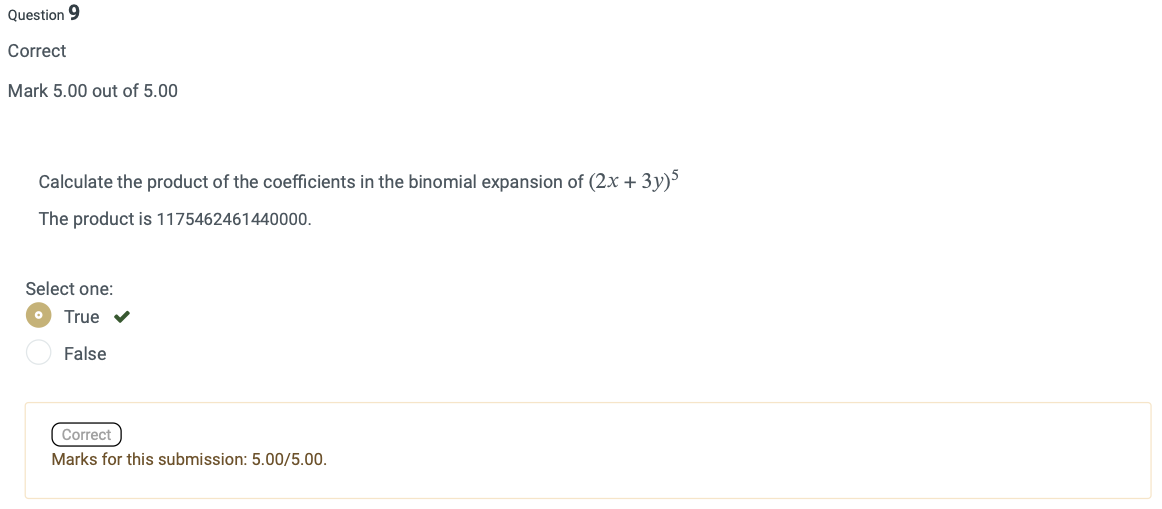
\includegraphics[width = 1.0\textwidth]{Images/Problem 9.png}
        \end{center}
    \end{Highlight}
\end{problem}

% Problem 9 Summary
\begin{summary}{Problem 9 Summary}
    \begin{statement}{Procedure}
        \begin{itemize}
            \item Modify the code from Problem 8 to multiply the coefficients of an expansion.
            \item Select the correct choice that corresponds with the result.
        \end{itemize}
    \end{statement}
    \begin{statement}{Key Concepts}
        \begin{itemize}
            \item This problem incorporates how to utilizes code for a Binomial Theorem algorithm so that it returns a different result.
        \end{itemize}
    \end{statement}
    \begin{statement}{Variations}
        \begin{itemize}
            \item We could be asked to calculate something different like the sum of coefficients.
            \begin{itemize}
                \item We would then slightly modify the algorithm so that it returns the result that is desired.
            \end{itemize}
        \end{itemize}
    \end{statement}
\end{summary}

% Problem 10
\begin{problem}{Problem 10}
    \begin{statement}{Problem Statement}
        Problem 10 from the mastery workbook quiz can be found on the following page.
    \end{statement}
    \begin{Highlight}[Solution]
        \begin{center}
            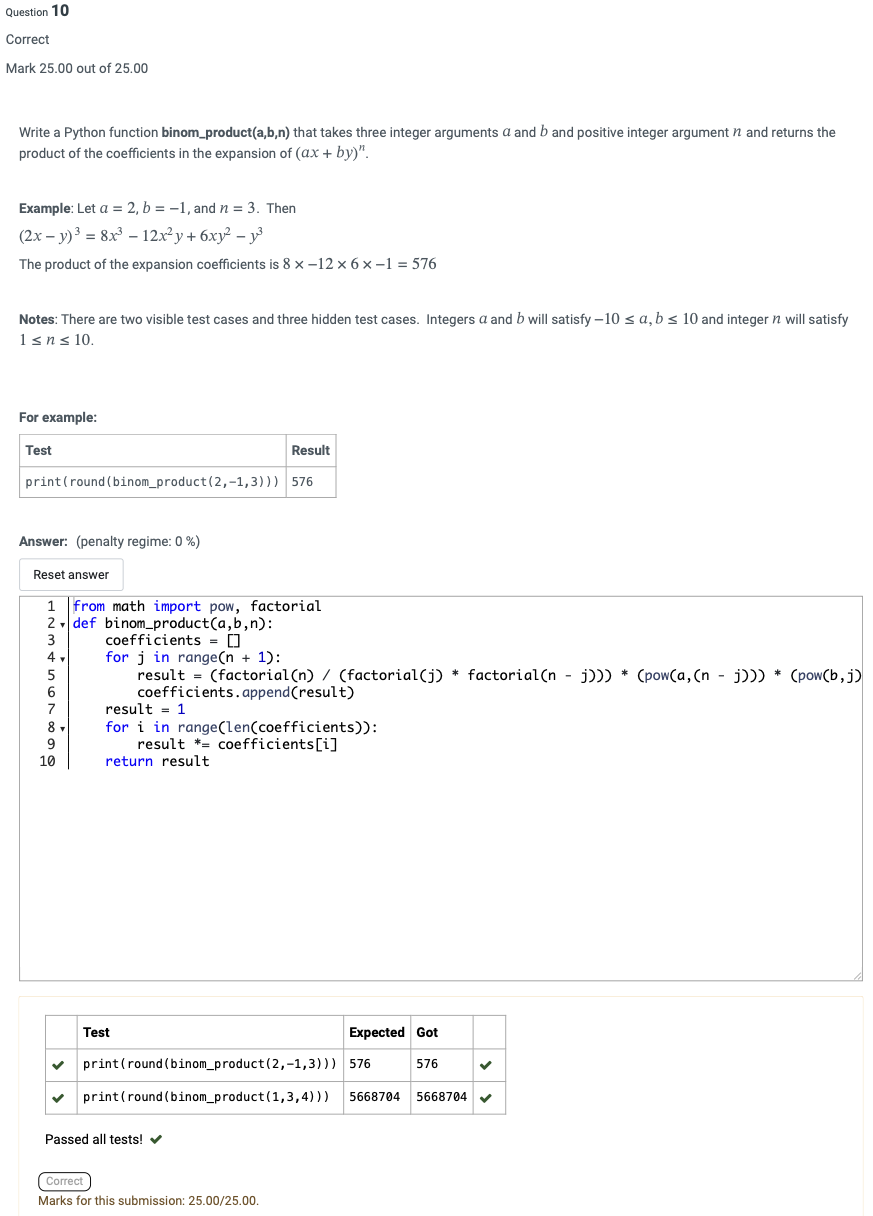
\includegraphics[width = 0.90\textwidth]{Images/Problem 10.png}
        \end{center}
    \end{Highlight}
\end{problem}

% Problem 10 Summary
\begin{summary}{Problem 10 Summary}
    \begin{statement}{Procedure}
        \begin{itemize}
            \item Write code in Python that achieves the result that we are seeking to produce.
        \end{itemize}
    \end{statement}
    \begin{statement}{Key Concepts}
        \begin{itemize}
            \item This problem incorporates the Binomial Theorem in the context of code in Python.
        \end{itemize}
    \end{statement}
    \begin{statement}{Variations}
        \begin{itemize}
            \item We could be asked to calculate something different with the coefficients of the expansion.
            \begin{itemize}
                \item We would then slightly modify the algorithm so that it achieves the result that we are seeking to have.
            \end{itemize}
        \end{itemize}
    \end{statement}
\end{summary}